\chapter{Clustering}


\section{PCA Clustering}
We decided to first try see if any of the digits would get separated using a PCA. We found that the digit 3 and 5 was somehow seperated into two classes with a few intermediate clusters.

\begin{figure}[H]
\centering
\includegraphics[width=1\linewidth]{code/pca_digit_cluster}
\caption{}
\label{fig:pca_cluster}
\end{figure}

In both cases this turned out to be a separation of whether the digits was bold or thin. In figure~\ref{fig:pca_cluster} the clusters can be seen separated by a low density region in the middle. We made the same plot with larger digits to show what meaning the PCA components had, but this means the clusters fade due to spacing between the digits. You can always open the PDF to inspect the numbers.

\begin{figure}[H]
\centering
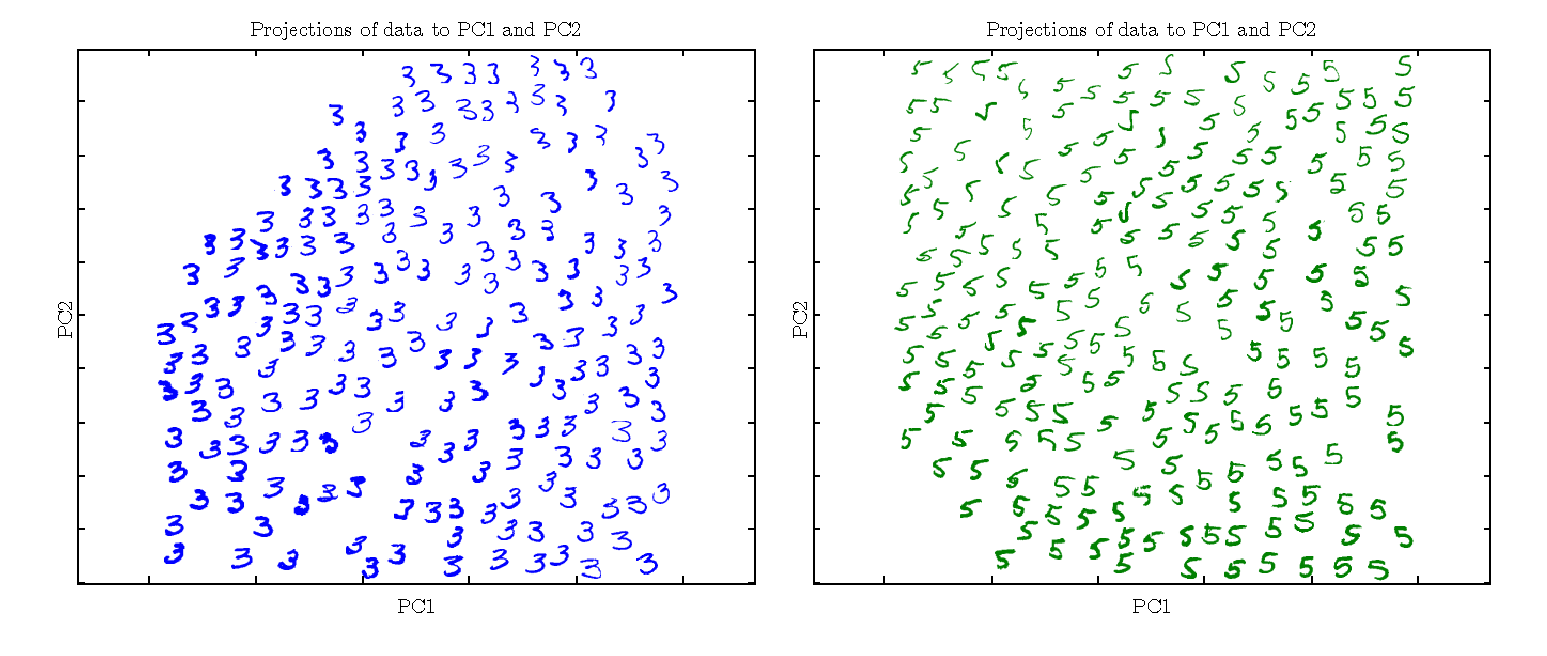
\includegraphics[width=1\linewidth]{code/pca_digit_cluster_z}
\caption{}
\label{fig:pca_cluster_zoom}
\end{figure}

\section{GMM}
